\documentclass[12pt,a4paper]{article}

\usepackage[romanian]{babel}
\usepackage{fontspec}
\usepackage{geometry}
\usepackage{graphicx}
\usepackage{float}
\usepackage{booktabs}
\usepackage{array}
\usepackage{hyperref}
\usepackage{xcolor}
\usepackage{enumitem}

\geometry{margin=2.5cm}
\hypersetup{
    colorlinks=true,
    linkcolor=blue!50!black,
    urlcolor=blue!50!black,
    citecolor=blue!50!black
}
\defaultfontfeatures{Ligatures=TeX}
\IfFontExistsTF{Arial}{
    \setmainfont{Arial}
    \setsansfont{Arial}
}{
    \setmainfont{TeX Gyre Heros}
    \setsansfont{TeX Gyre Heros}
}
\setmonofont{Menlo}
\definecolor{awdsnavy}{HTML}{002060}
\setlist{itemsep=0.25em, topsep=0.35em}

\begin{document}

\begin{titlepage}
\thispagestyle{empty}
\centering
\vspace*{2.2cm}
\begin{minipage}{0.30\textwidth}
    \centering
    
\includegraphics[height=3.0cm]{assets/poli_cover_logo.png}
\end{minipage}
\hfill
\begin{minipage}{0.48\textwidth}
    \centering
    
\includegraphics[height=3.0cm]{assets/acs_cover_logo.png}
\end{minipage}

\vspace{3.0cm}

{\sffamily\Large\color{awdsnavy} Raport cercetare semestrul 2\par}
\vspace{1.0cm}
{\sffamily\Huge\bfseries\color{awdsnavy} Adaptive Workplace Dynamics Simulator\par}
\vspace{0.35cm}
{\sffamily\Large\bfseries\color{awdsnavy} Simulare exploratorie agent-based a dinamicii organizaționale\par}

\vfill

\begin{minipage}{0.36\textwidth}
    \raggedright
    \sffamily
    Masterand:\par
    \vspace{0.25cm}
    \textbf{Pop Andrei}
\end{minipage}
\hfill
\begin{minipage}{0.36\textwidth}
    \raggedright
    \sffamily
    Îndrumător:\par
    \vspace{0.25cm}
    \textbf{Anca Andreea Morar}
\end{minipage}

\vspace{2.0cm}
{\sffamily\large 19 iunie 2026\par}
\end{titlepage}

\tableofcontents
\newpage

\section{Descriere tehnică și obiectiv}

AWDS este un prototip software pentru simularea exploratorie a unei organizații formate din agenți de tip angajat. Fiecare agent are o stare internă dinamică, care include stres, burnout, productivitate, stare emoțională, energie, satisfacție profesională, echilibru muncă--viață și engagement. Simularea avansează în pași discreți, fiecare pas reprezentând o zi de lucru.

Raportul se concentrează pe proiectarea și implementarea prototipului, nu pe o discuție teoretică extinsă despre comportamentul organizațional. Modelul este folosit ca instrument tehnic de experimentare: utilizatorul configurează parametri, rulează scenarii, compară traiectorii și exportă datele rezultate. Ieșirile sunt sintetice și trebuie citite ca rezultate interne ale modelului, nu ca date empirice despre organizații reale.

Obiectivul acestei etape este construirea unei platforme transparente, reproductibile și ușor de extins. Prototipul trebuie să permită comparații controlate între scenarii organizaționale, dar și comparații între două implementări ale aceleiași idei de model: un motor custom și un motor bazat pe Mesa. Accentul este pus pe fluxul tehnic complet: definirea parametrilor, execuția simulării, vizualizarea rezultatelor și exportul lor pentru raportare.

Din acest motiv, implementarea curentă urmărește patru cerințe principale:

\begin{itemize}
    \item configurarea clară a parametrilor organizaționali, personali, sociali și legați de evenimente;
    \item rulări reproductibile pe baza seed-urilor explicite și a presetărilor salvate;
    \item ieșiri comparabile între scenarii și între motoare;
    \item export de date și grafice care pot fi folosite în raportul de disertație.
\end{itemize}

\section{Funcționalități implementate}

Funcționalitățile implementate pot fi grupate în câteva zone principale:

\begin{itemize}
    \item configurarea numărului de agenți, zilelor simulate, seed-ului, presetărilor factory și presetărilor locale;
    \item controale pentru rulare, pauză/reluare, curățarea rezultatului și ajustarea intervalelor vizibile ale sliderelor;
    \item grafice live pentru stres, burnout, productivitate, stare emoțională, satisfacție, energie, turnover și distribuții finale;
    \item selector pentru motorul custom, motorul Mesa sau rularea ambelor motoare pentru comparație;
    \item istoric de rulări și export în formate JSON, CSV, TXT, PNG și ZIP.
\end{itemize}

\section{Modelul de simulare}

Fiecare pas al simulării reprezintă o zi de lucru. La fiecare zi, modelul aplică factori organizaționali, factori personali, influență socială, evenimente aleatoare și reguli de actualizare a stării fiecărui agent.

\subsection{Variabile și ipoteze}

Agenții sunt sintetici și sunt inițializați cu rol, reziliență, ambiție, nevoie de suport social, sensibilitate la navetă, încărcătură familială, variabilitate a sănătății, productivitate de bază, sensibilitate la stres și rată de recuperare. Variabilele urmărite sunt:

\begin{itemize}
    \item \textbf{stress}, \textbf{burnout}, \textbf{productivity}, \textbf{energy}, \textbf{satisfaction}, \textbf{work\_life\_balance} și \textbf{engagement}, normalizate între 0 și 1;
    \item \textbf{emotion}, între -1 și 1.
\end{itemize}

Modelul este intenționat simplificat: rețeaua socială rămâne statică pe durata unei rulări, evenimentele aleatoare sunt șocuri probabilistice, iar stilul de management și politica de lucru sunt modificatori de parametri. Stresul crește în funcție de cerințe și evenimente negative, dar scade prin resurse, recuperare și reziliență. Burnout-ul se acumulează mai lent, iar productivitatea poate crește la presiune moderată, dar scade la stres ridicat și burnout.

\subsection{Turnover}

În aplicație, \textit{turnover} înseamnă numărul cumulat de angajați simulați care părăsesc organizația. Plecarea unui agent poate apărea atunci când nivelul de burnout sau stres depășește pragurile configurate. Dacă înlocuirea este activă, un nou agent intră după o întârziere configurată și are temporar o penalizare de productivitate din cauza onboarding-ului.

\subsection{Reproductibilitate}

Același seed, aceeași configurație și același motor selectat duc la aceeași serie de rezultate pentru acel motor. Același seed nu produce neapărat traiectorii identice între motorul custom și Mesa, deoarece implementarea și ordinea de activare sunt diferite.

\section{Implementare tehnică}

Aplicația este implementată în Python. Interfața web este realizată cu Streamlit, calculele numerice cu NumPy, datele sunt organizate/exportate cu Pandas, graficele exportabile sunt generate cu Matplotlib, iar graficele interactive folosesc Plotly. Implementarea Mesa folosește clasele de model și agent din Mesa împreună cu un spațiu de rețea bazat pe NetworkX.

\subsection{Arhitectura motoarelor de simulare}

Prototipul separă acum logica de simulare în spatele unei interfețe de motor. Un motor expune aceleași operații de bază: avansarea cu o zi, rularea până la final, întoarcerea unui snapshot live și întoarcerea rezultatului final. Dashboard-ul folosește \texttt{engines.py} pentru a mapa numele motorului selectat la implementarea care trebuie rulată. Astfel, interfața nu depinde de implementarea exactă a motorului.

Motorul custom, implementat în \texttt{engine.py}, gestionează direct lista de agenți, rețeaua socială, evenimentele aleatoare, actualizările zilnice, turnover-ul, înlocuirile și metricile agregate. Avantajul principal este transparența: ecuațiile de actualizare și formatul ieșirilor sunt ușor de inspectat.

\subsection{Alternativa Mesa}

Mesa a fost adăugat ca motor alternativ în \texttt{mesa\_engine.py}. În această versiune, mediul de lucru este reprezentat ca model Mesa, angajații sunt agenți Mesa, iar relațiile sunt stocate într-un network grid bazat pe NetworkX. Motorul Mesa păstrează aceleași câmpuri de rezultat ca motorul custom, astfel încât dashboard-ul, exporturile și tabelele comparative pot trata uniform ambele motoare.

Scopul adăugării Mesa nu este obținerea unor rezultate identice, ci compararea tendințelor în două implementări. Ambele motoare întorc aceeași schemă de ieșire: configurație, serie temporală agregată, stări finale, jurnal de evenimente și sumar final. Astfel, dashboard-ul, exporturile și tabelele comparative reutilizează același cod.

\subsection{Fluxul dashboard-ului și al exporturilor}

Dashboard-ul Streamlit susține fluxul de lucru exploratoriu: alegerea unei presetări, ajustarea parametrilor, rularea simulării, compararea scenariilor și exportul rezultatelor. După finalizarea unei rulări, interfața afișează metrici sumar, grafice de tip serie temporală și distribuții finale.

\subsection{Interfața aplicației}

Interfața aplicației este organizată astfel încât configurarea, rularea și interpretarea rezultatelor să fie disponibile în același flux de lucru. Sidebar-ul conține presetările, controalele de rulare și parametrii principali ai modelului, iar zona centrală afișează tab-urile pentru rulare, comparare, export și descrierea modelului.

\begin{figure}[H]
    \centering
    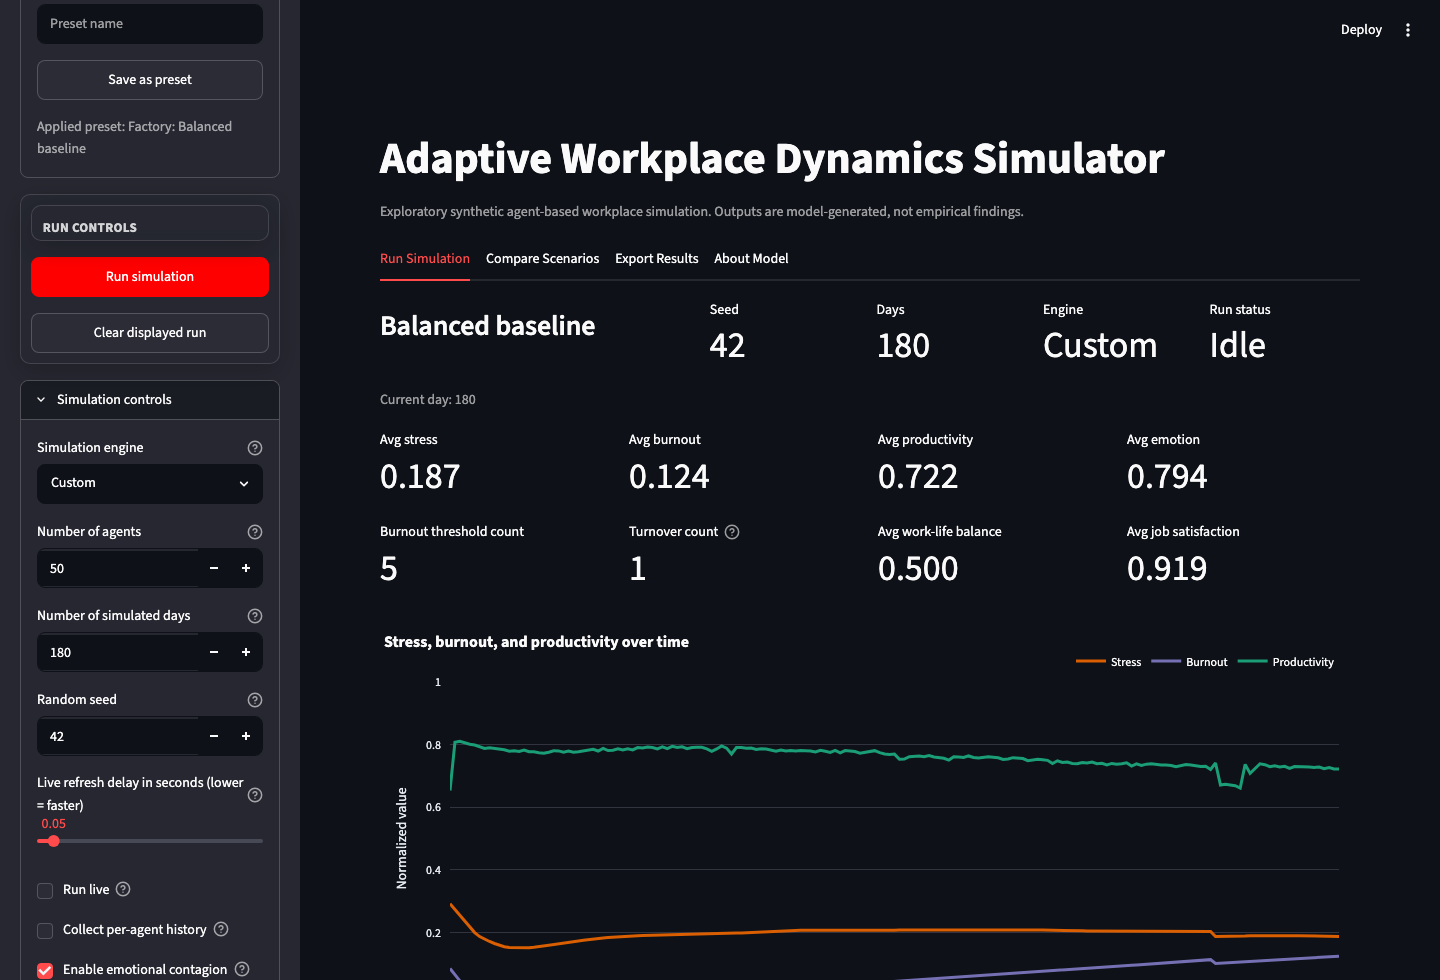
\includegraphics[width=\textwidth]{figures/ro_app_run_dashboard.png}
    \caption{Tab-ul \textit{Run Simulation} după rularea scenariului baseline.}
\end{figure}

Tab-ul de comparare rulează aceleași presetări cu aceeași configurație globală și afișează rezultatele într-un tabel agregat. Această vedere este utilă pentru inspectarea rapidă a diferențelor dintre scenarii înainte de exportul datelor.

\begin{figure}[H]
    \centering
    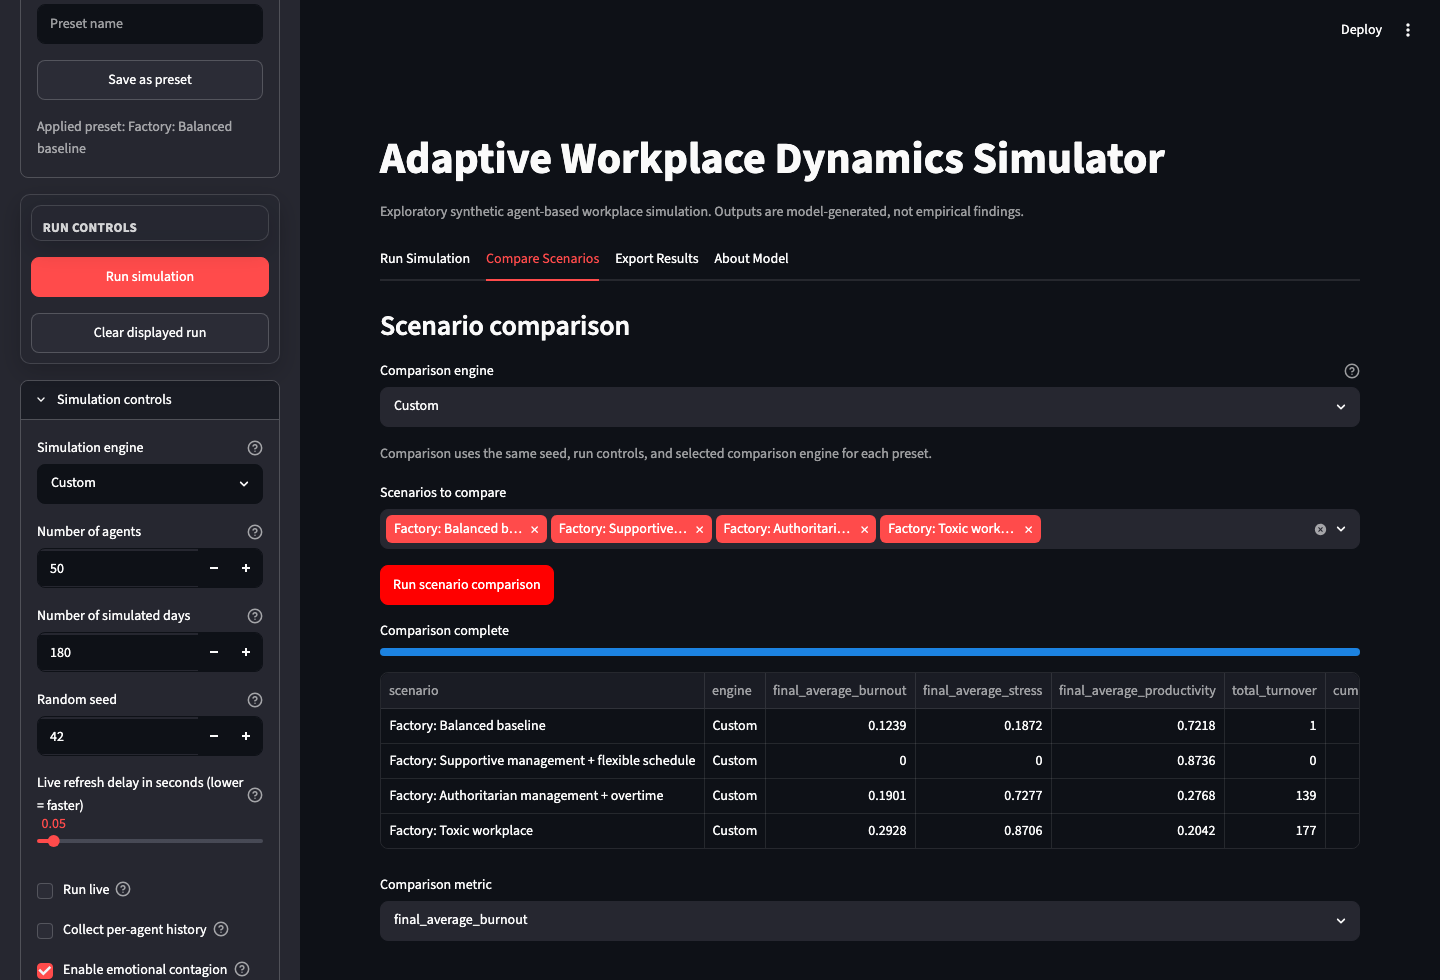
\includegraphics[width=\textwidth]{figures/ro_app_comparison_tab.png}
    \caption{Tab-ul \textit{Compare Scenarios} după finalizarea unei comparații de scenarii.}
\end{figure}

\section{Scenarii și rezultate}
\label{sec:rezultate}

Această secțiune prezintă o rulare comparativă a presetărilor principale din prototip. Scopul ei este să demonstreze fluxul tehnic de analiză, nu să stabilească o concluzie empirică despre mediile de lucru reale.

Fluxul de comparație este central pentru prototip. Scenariile pot fi comparate cu motorul custom, cu motorul Mesa sau cu ambele motoare. Astfel se obține o imagine mai clară asupra întrebării de cercetare: dacă efectul observat ține de scenariu sau de diferențele introduse de motorul de simulare.

\subsection{Design experimental}

Au fost selectate patru presetări: baseline, suportiv + flexibil, autoritar + overtime și toxic. Ele acoperă un caz neutru, unul favorabil și două cazuri de presiune ridicată. Pentru fiecare rulare s-au păstrat constante numărul de agenți, numărul de zile, seed-ul și controalele generale, schimbând doar presetarea și motorul de simulare.

Metricile urmărite sunt stresul final, burnout-ul final, productivitatea finală, turnover-ul și burnout-ul cumulativ. Ele trebuie citite ca indicatori interni ai modelului, utili pentru compararea scenariilor sintetice, nu ca valori empirice despre organizații reale.

\subsection{Configurația experimentală}

\begin{itemize}
    \item Număr agenți: 50
    \item Număr zile simulate: 180
    \item Seed folosit: 20260618
    \item Motoare comparate: Custom și Mesa
    \item Scenarii comparate: Balanced baseline, Supportive management + flexible schedule, Authoritarian management + overtime și Toxic workplace
    \item Parametri modificați față de presetări: niciunul; s-au păstrat constante controalele globale ale rulării.
\end{itemize}

Datele brute pentru această secțiune au fost exportate ca fișiere CSV în directorul \texttt{data/} al raportului. Turnover-ul este raportat ca număr cumulat de plecări pe durata rulării. Deoarece înlocuirea angajaților este activă, valoarea poate depăși numărul inițial de agenți în scenariile severe.

\subsection{Tabel comparativ}

\begin{table}[H]
    \centering
    \resizebox{\textwidth}{!}{%
    \begin{tabular}{llrrrrr}
        \toprule
        Scenariu & Motor & Stres final & Burnout final & Productivitate finală & Turnover & Burnout cumulativ \\
        \midrule
        Baseline & Custom & 0.144 & 0.078 & 0.758 & 4 & 8.56 \\
        Baseline & Mesa & 0.182 & 0.096 & 0.744 & 2 & 7.57 \\
        Suportiv + flexibil & Custom & 0.000 & 0.000 & 0.872 & 0 & 0.20 \\
        Suportiv + flexibil & Mesa & 0.000 & 0.000 & 0.863 & 0 & 0.21 \\
        Autoritar + overtime & Custom & 0.780 & 0.257 & 0.228 & 132 & 41.69 \\
        Autoritar + overtime & Mesa & 0.829 & 0.202 & 0.244 & 121 & 45.40 \\
        Toxic & Custom & 0.894 & 0.302 & 0.181 & 188 & 50.05 \\
        Toxic & Mesa & 0.877 & 0.258 & 0.185 & 185 & 54.95 \\
        \bottomrule
    \end{tabular}
    }
    \caption{Rezultate sintetice comparative obținute din simulările AWDS pentru 50 de agenți, 180 de zile și seed-ul 20260618.}
\end{table}

\subsection{Grafic sumar}

\begin{figure}[H]
    \centering
    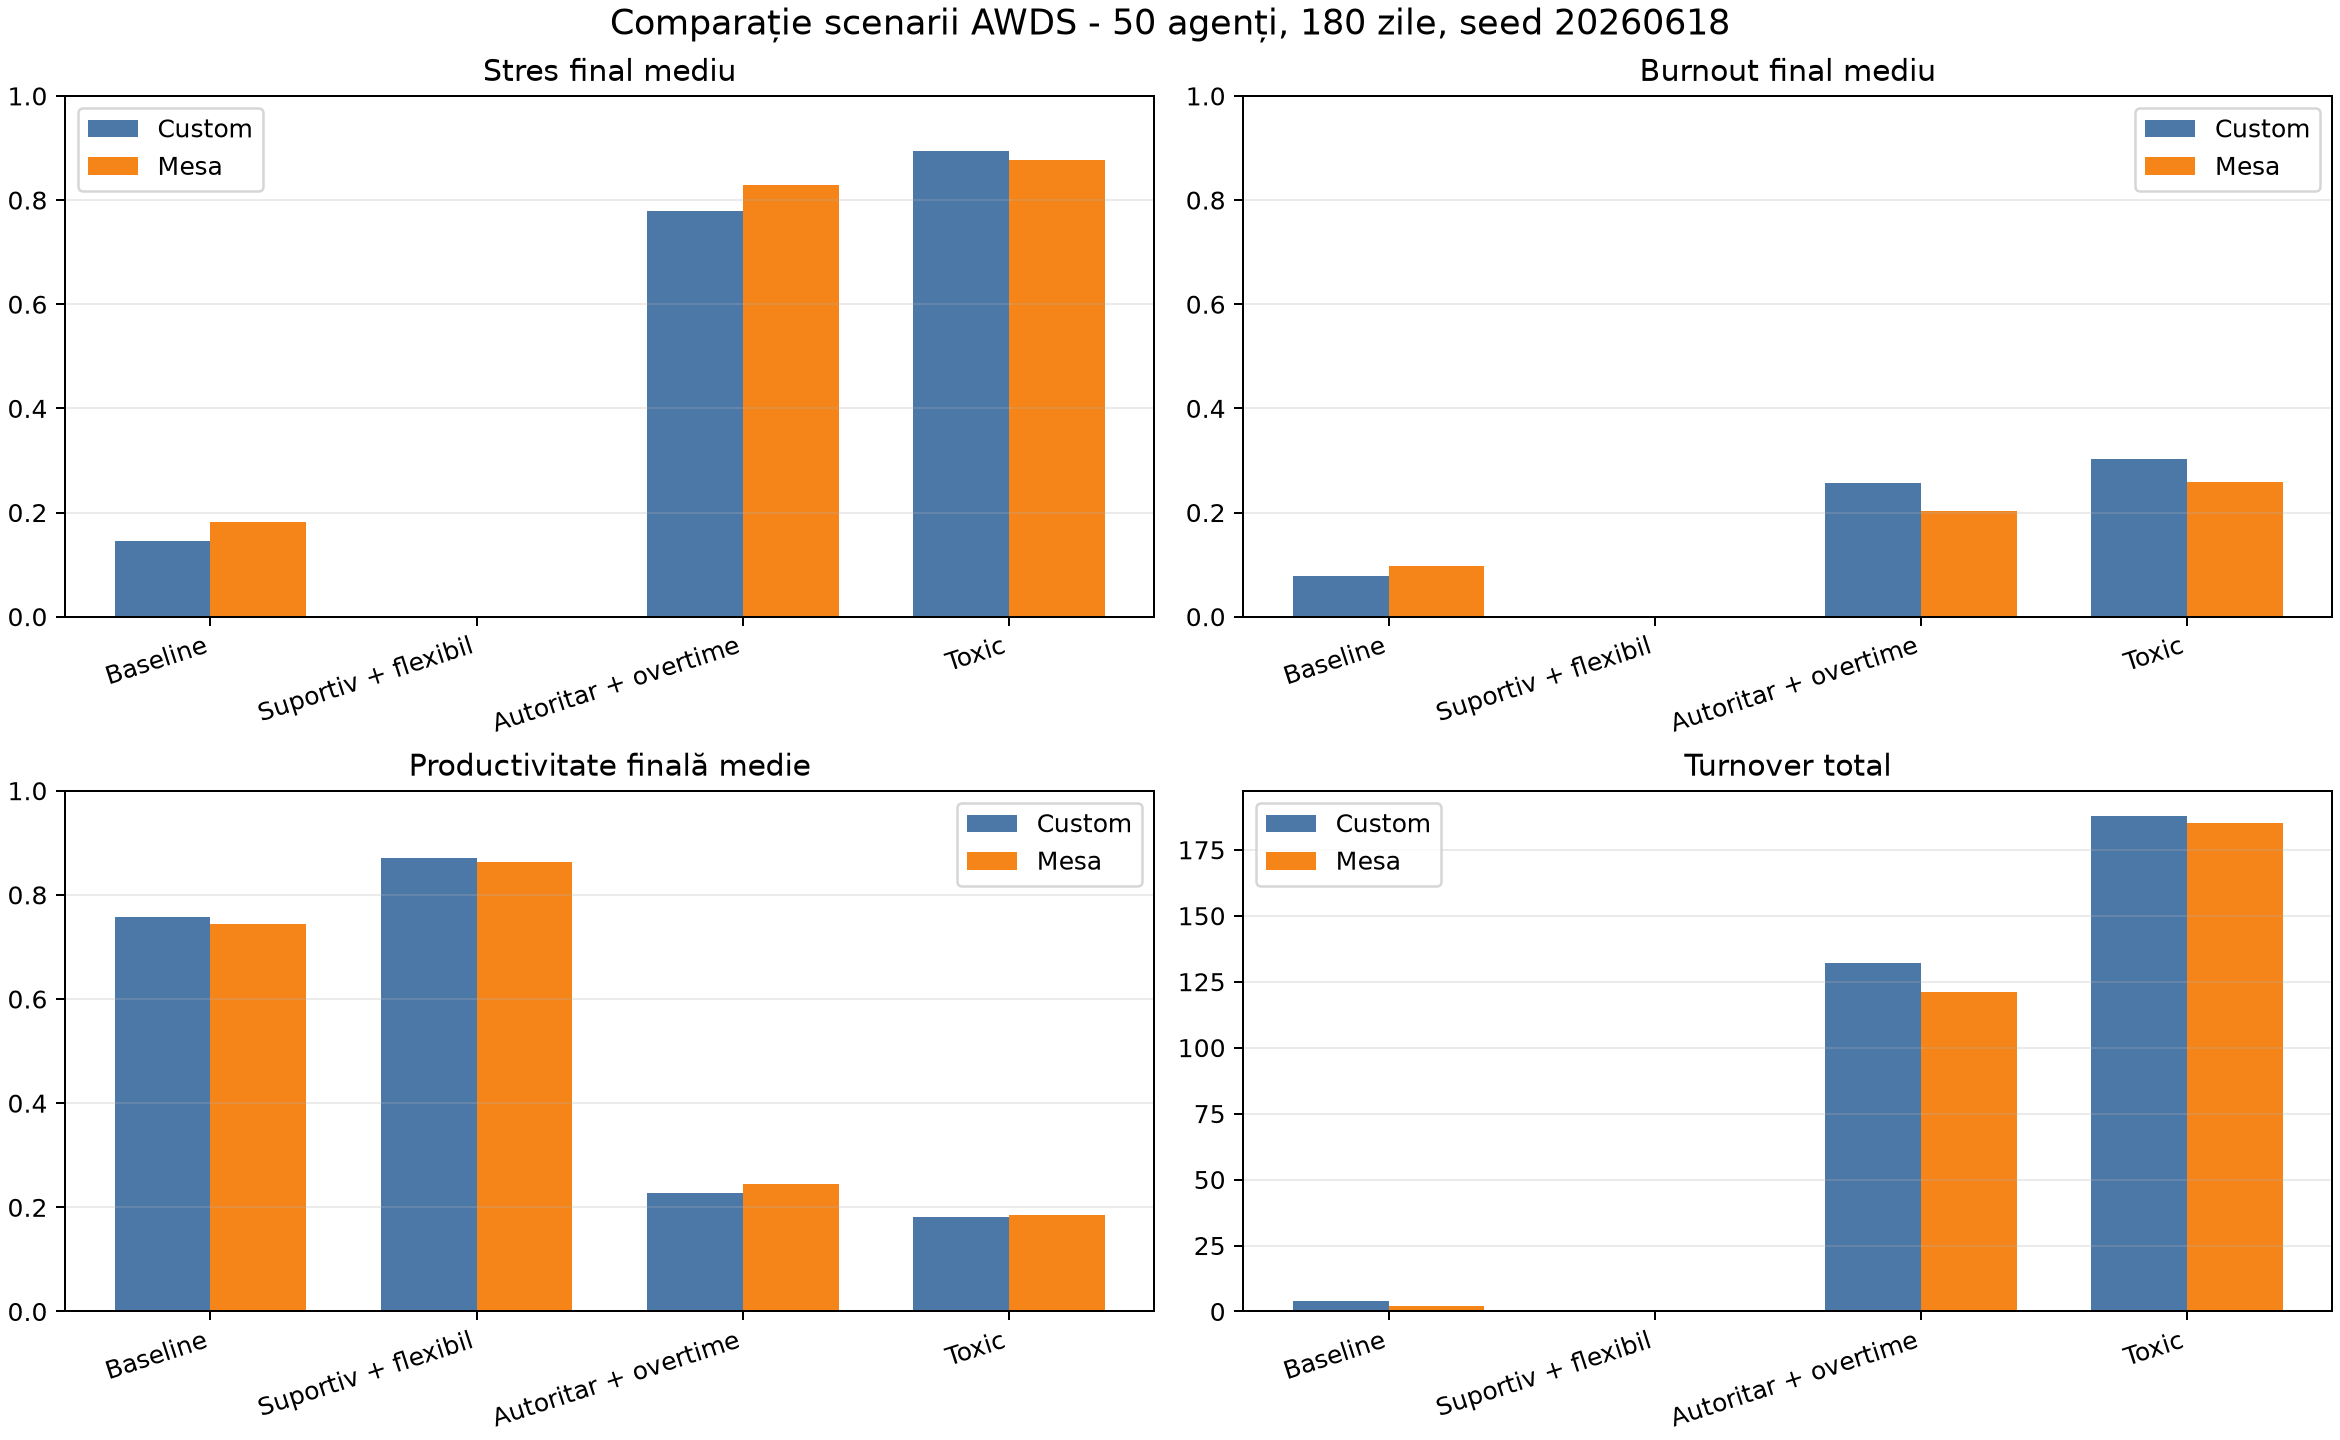
\includegraphics[width=0.92\textwidth]{figures/ro_section6_comparison_summary.png}
    \caption{Comparație finală între scenariile AWDS și cele două motoare de simulare.}
\end{figure}

\begin{figure}[H]
    \centering
    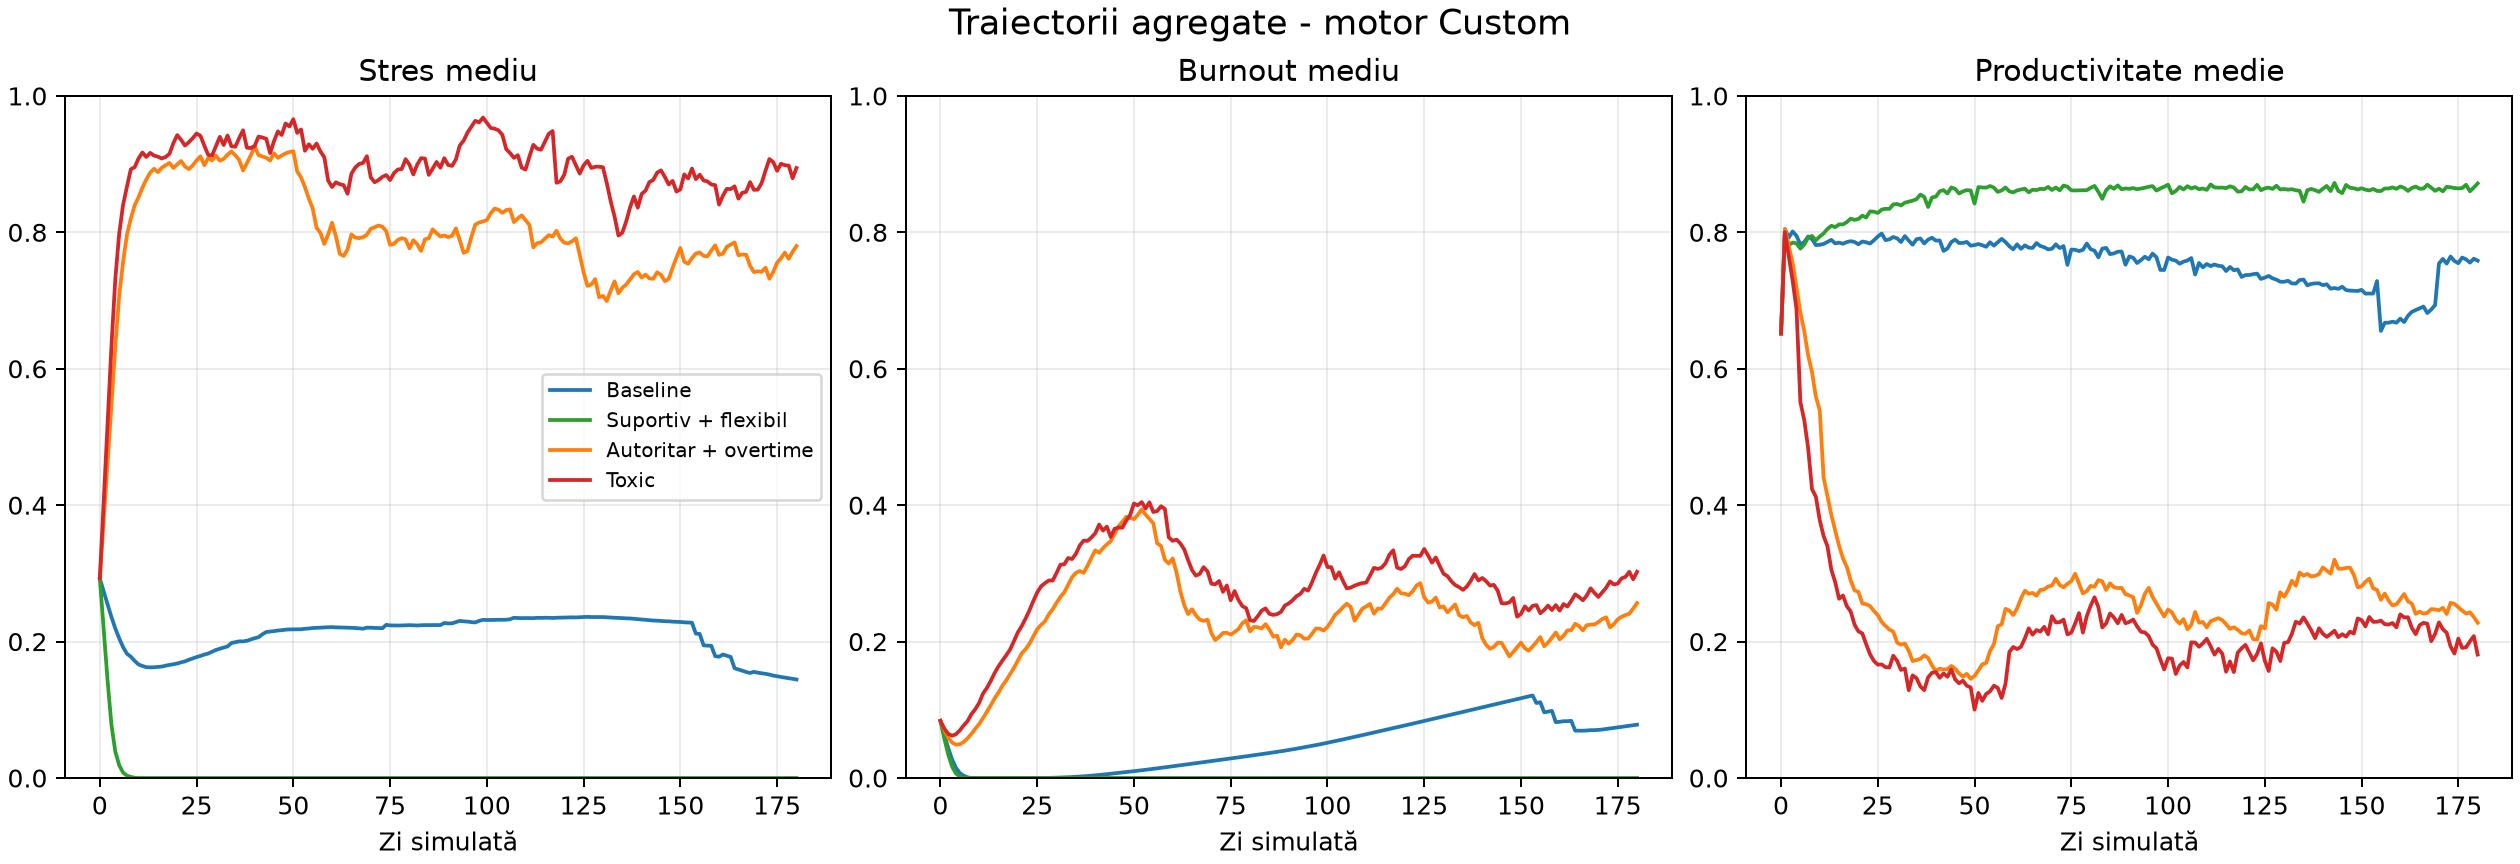
\includegraphics[width=0.92\textwidth]{figures/ro_section6_timeseries_custom.png}
    \caption{Traiectorii agregate pentru scenariile rulate cu motorul custom.}
\end{figure}

\begin{figure}[H]
    \centering
    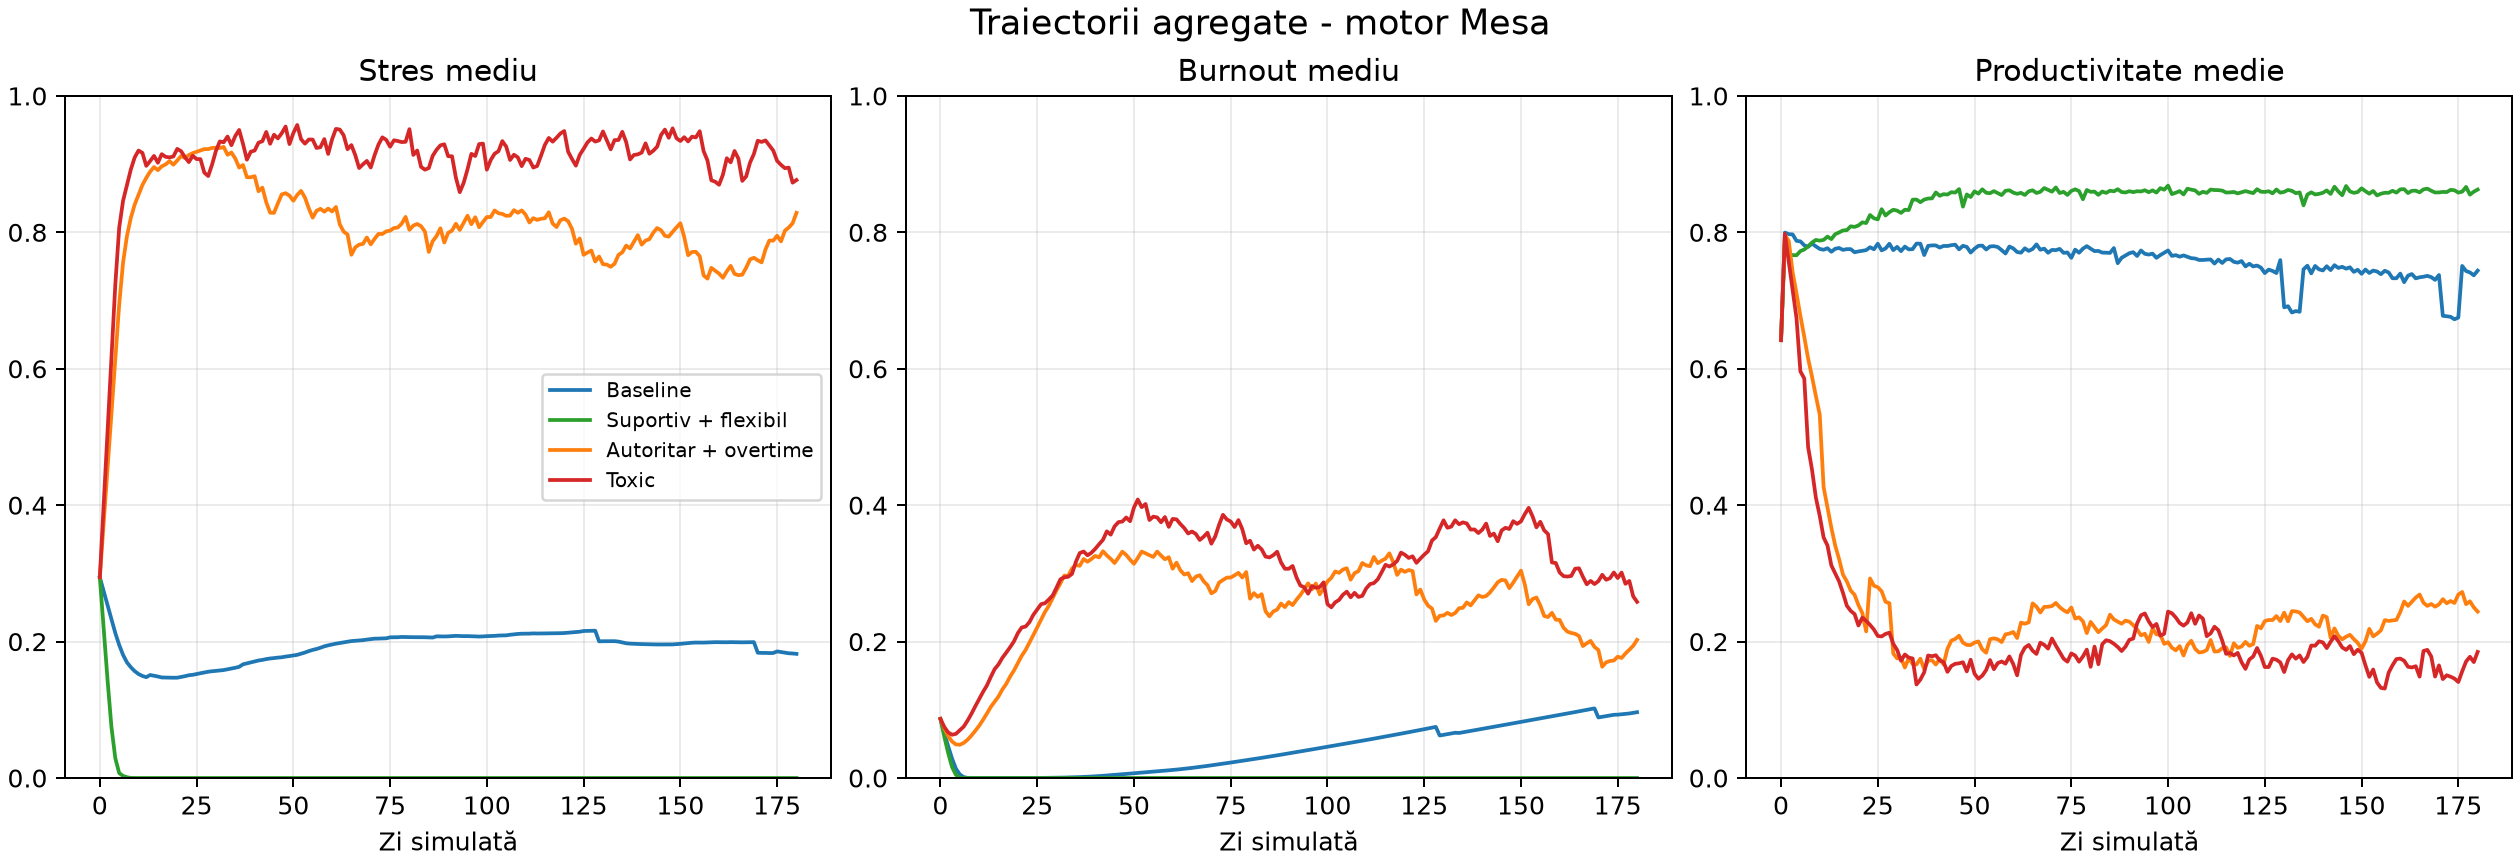
\includegraphics[width=0.92\textwidth]{figures/ro_section6_timeseries_mesa.png}
    \caption{Traiectorii agregate pentru scenariile rulate cu motorul Mesa.}
\end{figure}

\subsection{Interpretare}

Rezultatele separă clar scenariul suportiv de cele cu presiune ridicată. \textit{Supportive management + flexible schedule} menține stresul și burnout-ul aproape de zero și păstrează productivitatea ridicată. În schimb, \textit{Authoritarian management + overtime} și \textit{Toxic workplace} cresc stresul, reduc productivitatea și generează turnover cumulat mare.

Turnover-ul poate depăși numărul inițial de agenți deoarece înlocuirea este activă: un angajat plecat este înlocuit, iar înlocuitorul poate pleca la rândul lui. Compararea motoarelor arată aceeași direcție generală a rezultatelor, chiar dacă valorile nu sunt identice, ceea ce susține fluxul tehnic de comparație fără a valida empiric modelul.

\section{Dificultăți întâmpinate}

Principala dificultate a fost proiectarea unui model suficient de expresiv încât să nu reducă dinamica organizațională la reguli triviale. Modelul trebuia să permită situații nuanțate: presiunea moderată poate crește productivitatea pe termen scurt, în timp ce presiunea ridicată și susținută poate produce burnout și scădere de performanță.

O altă dificultate a fost balansarea parametrilor astfel încât scenariile să producă diferențe vizibile fără să ajungă imediat în extreme. A fost necesară separarea între stres, burnout, energie, satisfacție și productivitate, deoarece aceste variabile nu se mișcă toate cu aceeași viteză și nu răspund identic la aceiași factori.

La nivel tehnic, interfața, exporturile și al doilea motor au trebuit aliniate la aceeași schemă de ieșire. Astfel, graficele, istoricul rulărilor și tabelele comparative pot folosi același cod indiferent dacă rezultatul vine din motorul custom sau din Mesa.

\section{Limitări}

Modelul folosește date sintetice și nu este calibrat pe date empirice reale. Relațiile sociale sunt reprezentate printr-o rețea statică, evenimentele sunt probabilistice, iar trăsăturile agenților sunt generate din distribuții simple. Rezultatele pot descrie comportamentul intern al prototipului, dar nu pot fi tratate ca dovezi despre companii reale.

\section{Direcții viitoare}

Direcția cea mai importantă este calibrarea modelului pe date reale, de exemplu printr-un formular despre stres perceput, volum de lucru, suport managerial, autonomie, echilibru muncă--viață, satisfacție și intenția de a părăsi organizația. Aceste răspunsuri ar permite ajustarea parametrilor și compararea tendințelor sintetice cu date anonimizate.

\begin{itemize}
    \item calibrarea parametrilor pe baza răspunsurilor colectate;
    \item analiza de sensibilitate pentru a vedea ce parametri influențează cel mai mult rezultatele;
    \item extinderea modelului cu echipe, departamente și roluri organizaționale;
    \item salvarea persistentă a rulărilor și generarea automată de rapoarte.
\end{itemize}

\section{Demo video}

Demo-ul video prezintă pornirea aplicației, aplicarea unei presetări, rularea unei simulări, compararea scenariilor cu motoarele disponibile și exportul rezultatelor în formatele generate de prototip.

Link demo video: \textit{[de completat]}

\end{document}
